
\begin{figure}[h]
\centering
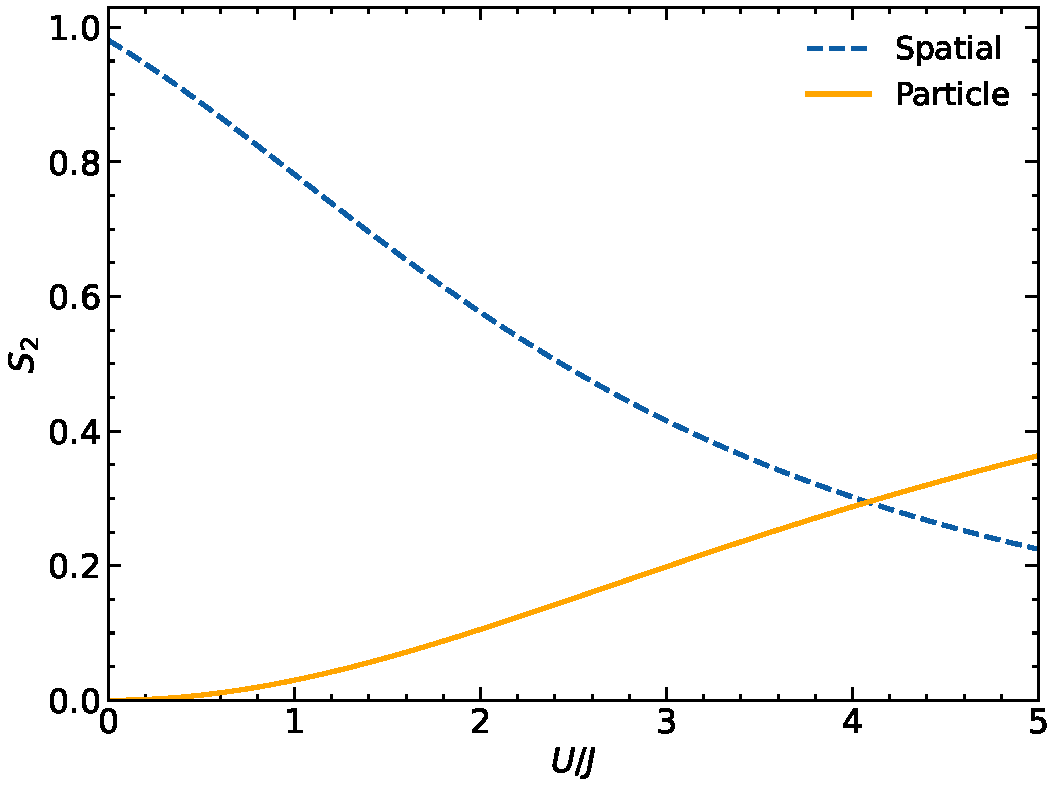
\includegraphics[scale=0.5]{../figures/ed_renyi.pdf}
\caption{The figure above is a graph of the Renyi entanglement entropy for both spatial and particle bipartitions versus the ratio of the interaction term to the hopping term.}
\end{figure}

\subsection{PIGSFLI Algorithm}

A Monte Carlo simulation is a stochastic (random) method of integration, which allows for accurate estimations of desired values. Monte Carlo is necessary for situations where exact calculations are too computationally expensive, such as in the exact diagonalization of the reduced density matrix for high particle/site number Bose Hubbard systems. The size of the Hilbert space is calculated by \cref{eq:36} and shown by \cref{fig:hilbert_space_size}:

\begin{equation}
D = \frac{\left(N+L-1\right)!}{\left(N\right)!\left(L-1\right)!}
\label{eq:36}
\end{equation}

\begin{figure}[h]
\centering
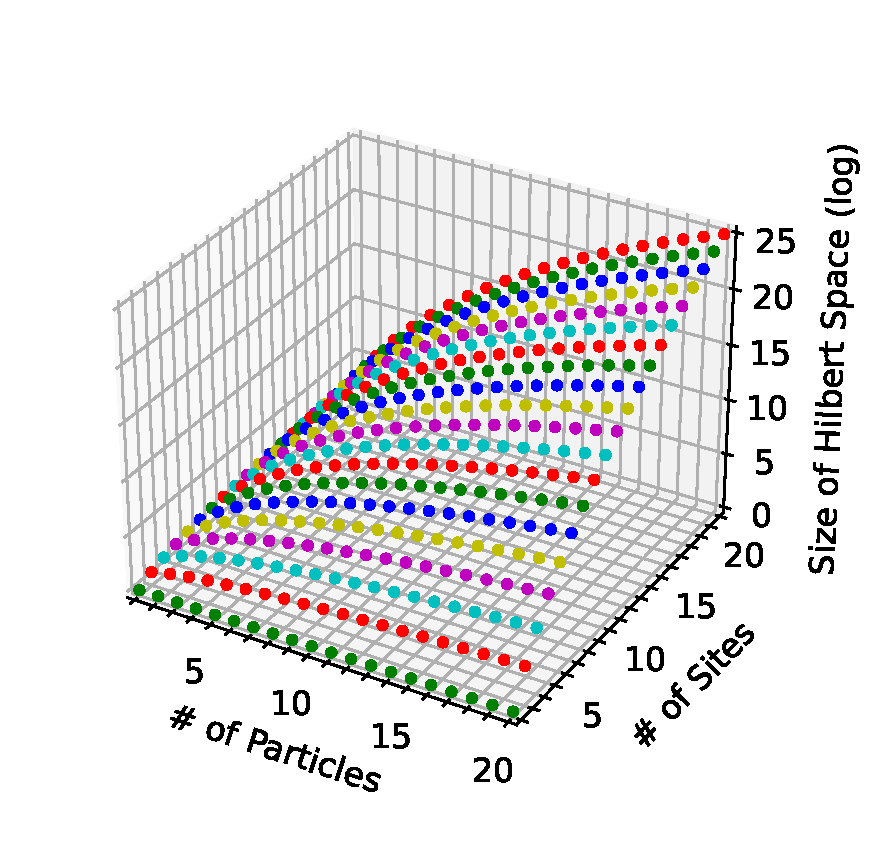
\includegraphics[scale=0.5]{../figures/hilbert_space_size.pdf}
\caption{The figure above shows the size of the Hilbert space as a function of number of sites and particles. This 3-dimensional plot for the number of combinations in the Hilbert space goes up to $20$ sites and $20$ particles.}
\label{fig:hilbert_space_size}
\end{figure}


\begin{figure}
\centering
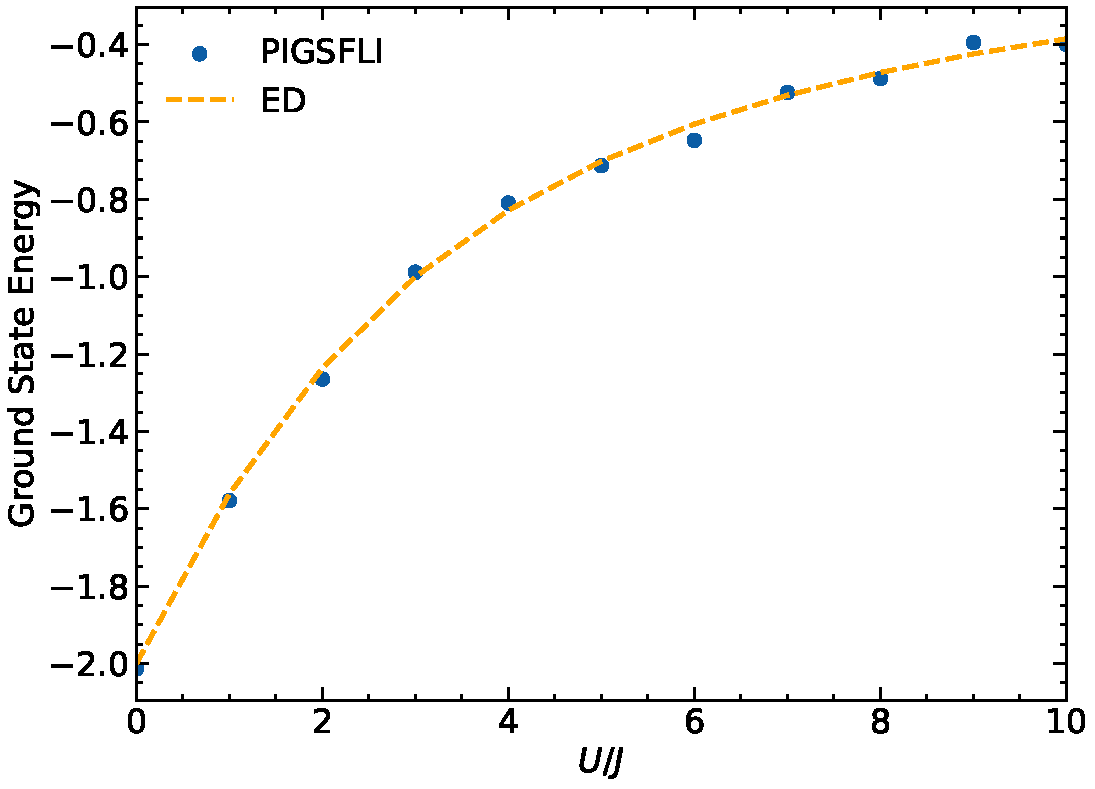
\includegraphics[scale=0.5]{../figures/total_energy.pdf}
\caption{A plot of the ground state energy versus the ratio between U, the potential term, and J, the hopping term for both exact diagonalization and PIGSFLI algorithm. From this plot, the PIGSFLI reults match very well to our ED calculation.}
\label{fig:total_energy}
\end{figure}

\begin{figure}
\centering
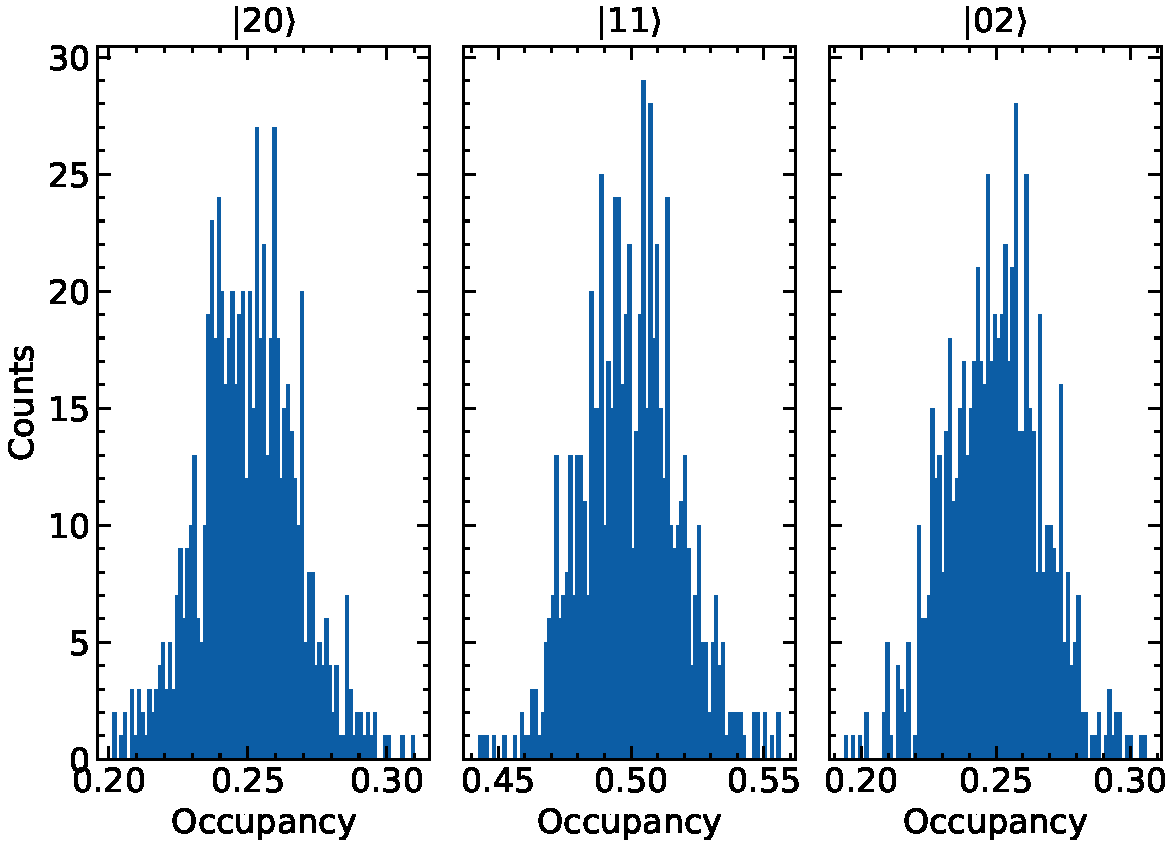
\includegraphics[scale=0.5]{../figures/sep_occ_hist_U_0.0001.pdf}
\caption{The figure above shows the histogram of the occupation number for the particle bipartition as a function of the ratio of the interaction term to the hopping term. This graph specifically shows the case where the interaction term is $10$ times the hopping term.}
\label{fig:sep_occ_hist_U_0.0001}
\end{figure}

\begin{figure}
\centering
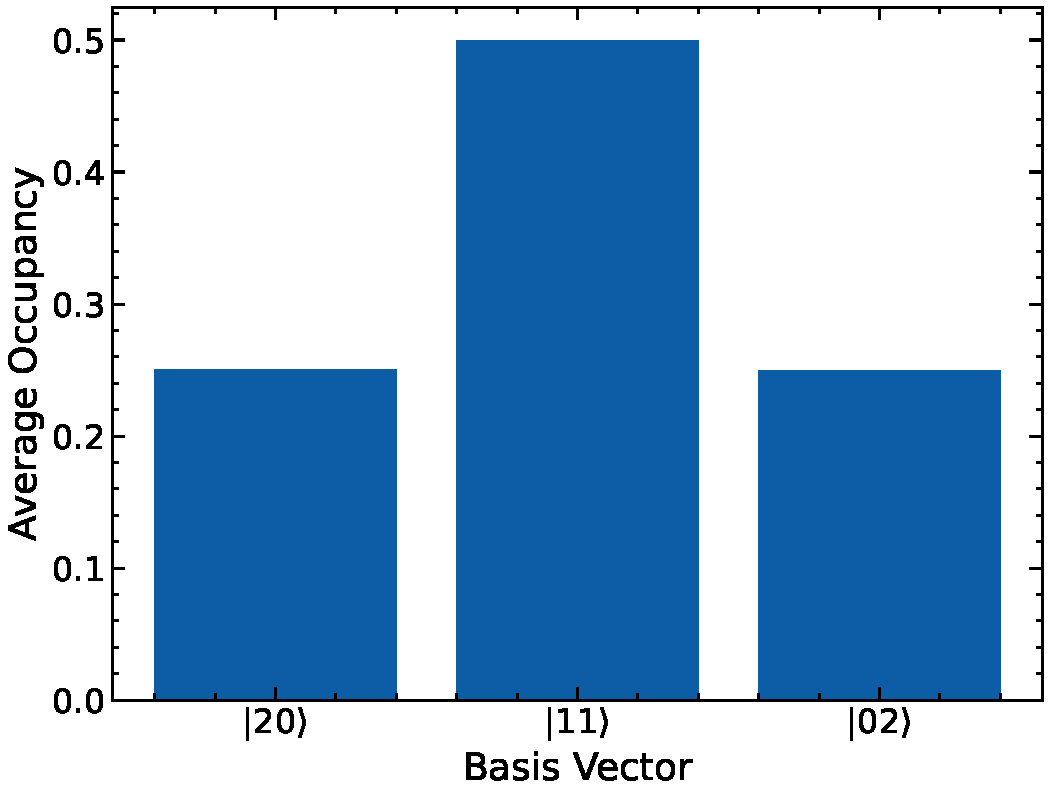
\includegraphics[scale=0.5]{../figures/spatial_avg_occ_U_0.0001.pdf}
\caption{The figure above shows the average occupation number for the spatial bipartition as a function of the ratio of the interaction term to the hopping term. This graph specifically shows the case where the interaction term is $10$ times the hopping term.}
\label{fig:spatial_avg_occ_U_0.0001}
\end{figure}

\begin{figure}
\centering
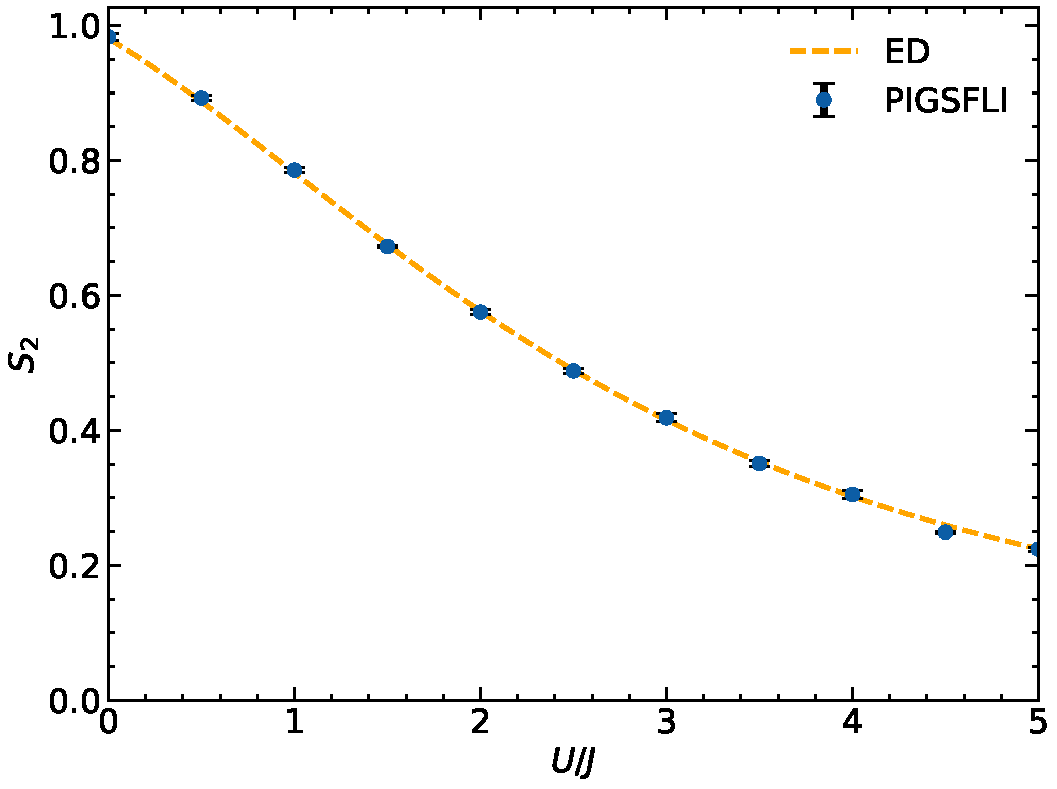
\includegraphics[scale=0.5]{../figures/renyi_spatial.pdf}
\caption{The second Rényi spatial entanglement entropy as a function of U/J for both exact diagonalization (ED) and PIGSFLI. This plot shows excellent agreement between the PIGSFLI estimation and that of our ED calculation, showing that PIGSFLI is a viable option for computation on much larger system sizes.}
\label{fig:renyi_spatial}
\end{figure}